\documentclass{article}

\usepackage{graphicx}
\usepackage{tikz}
\usepackage{tikzsymbols}
\usetikzlibrary{calc,patterns,shapes.geometric}
\pagestyle{empty}
\usepackage[margin=0pt]{geometry}
\geometry{papersize={14in,12in}}

\def\centerarc[#1](#2)(#3:#4:#5){\draw[#1] ($(#2)+({#5*cos(#3)},{#5*sin(#3)})$) arc (#3:#4:#5);}

\begin{document}
	\begin{figure}
		\centering
		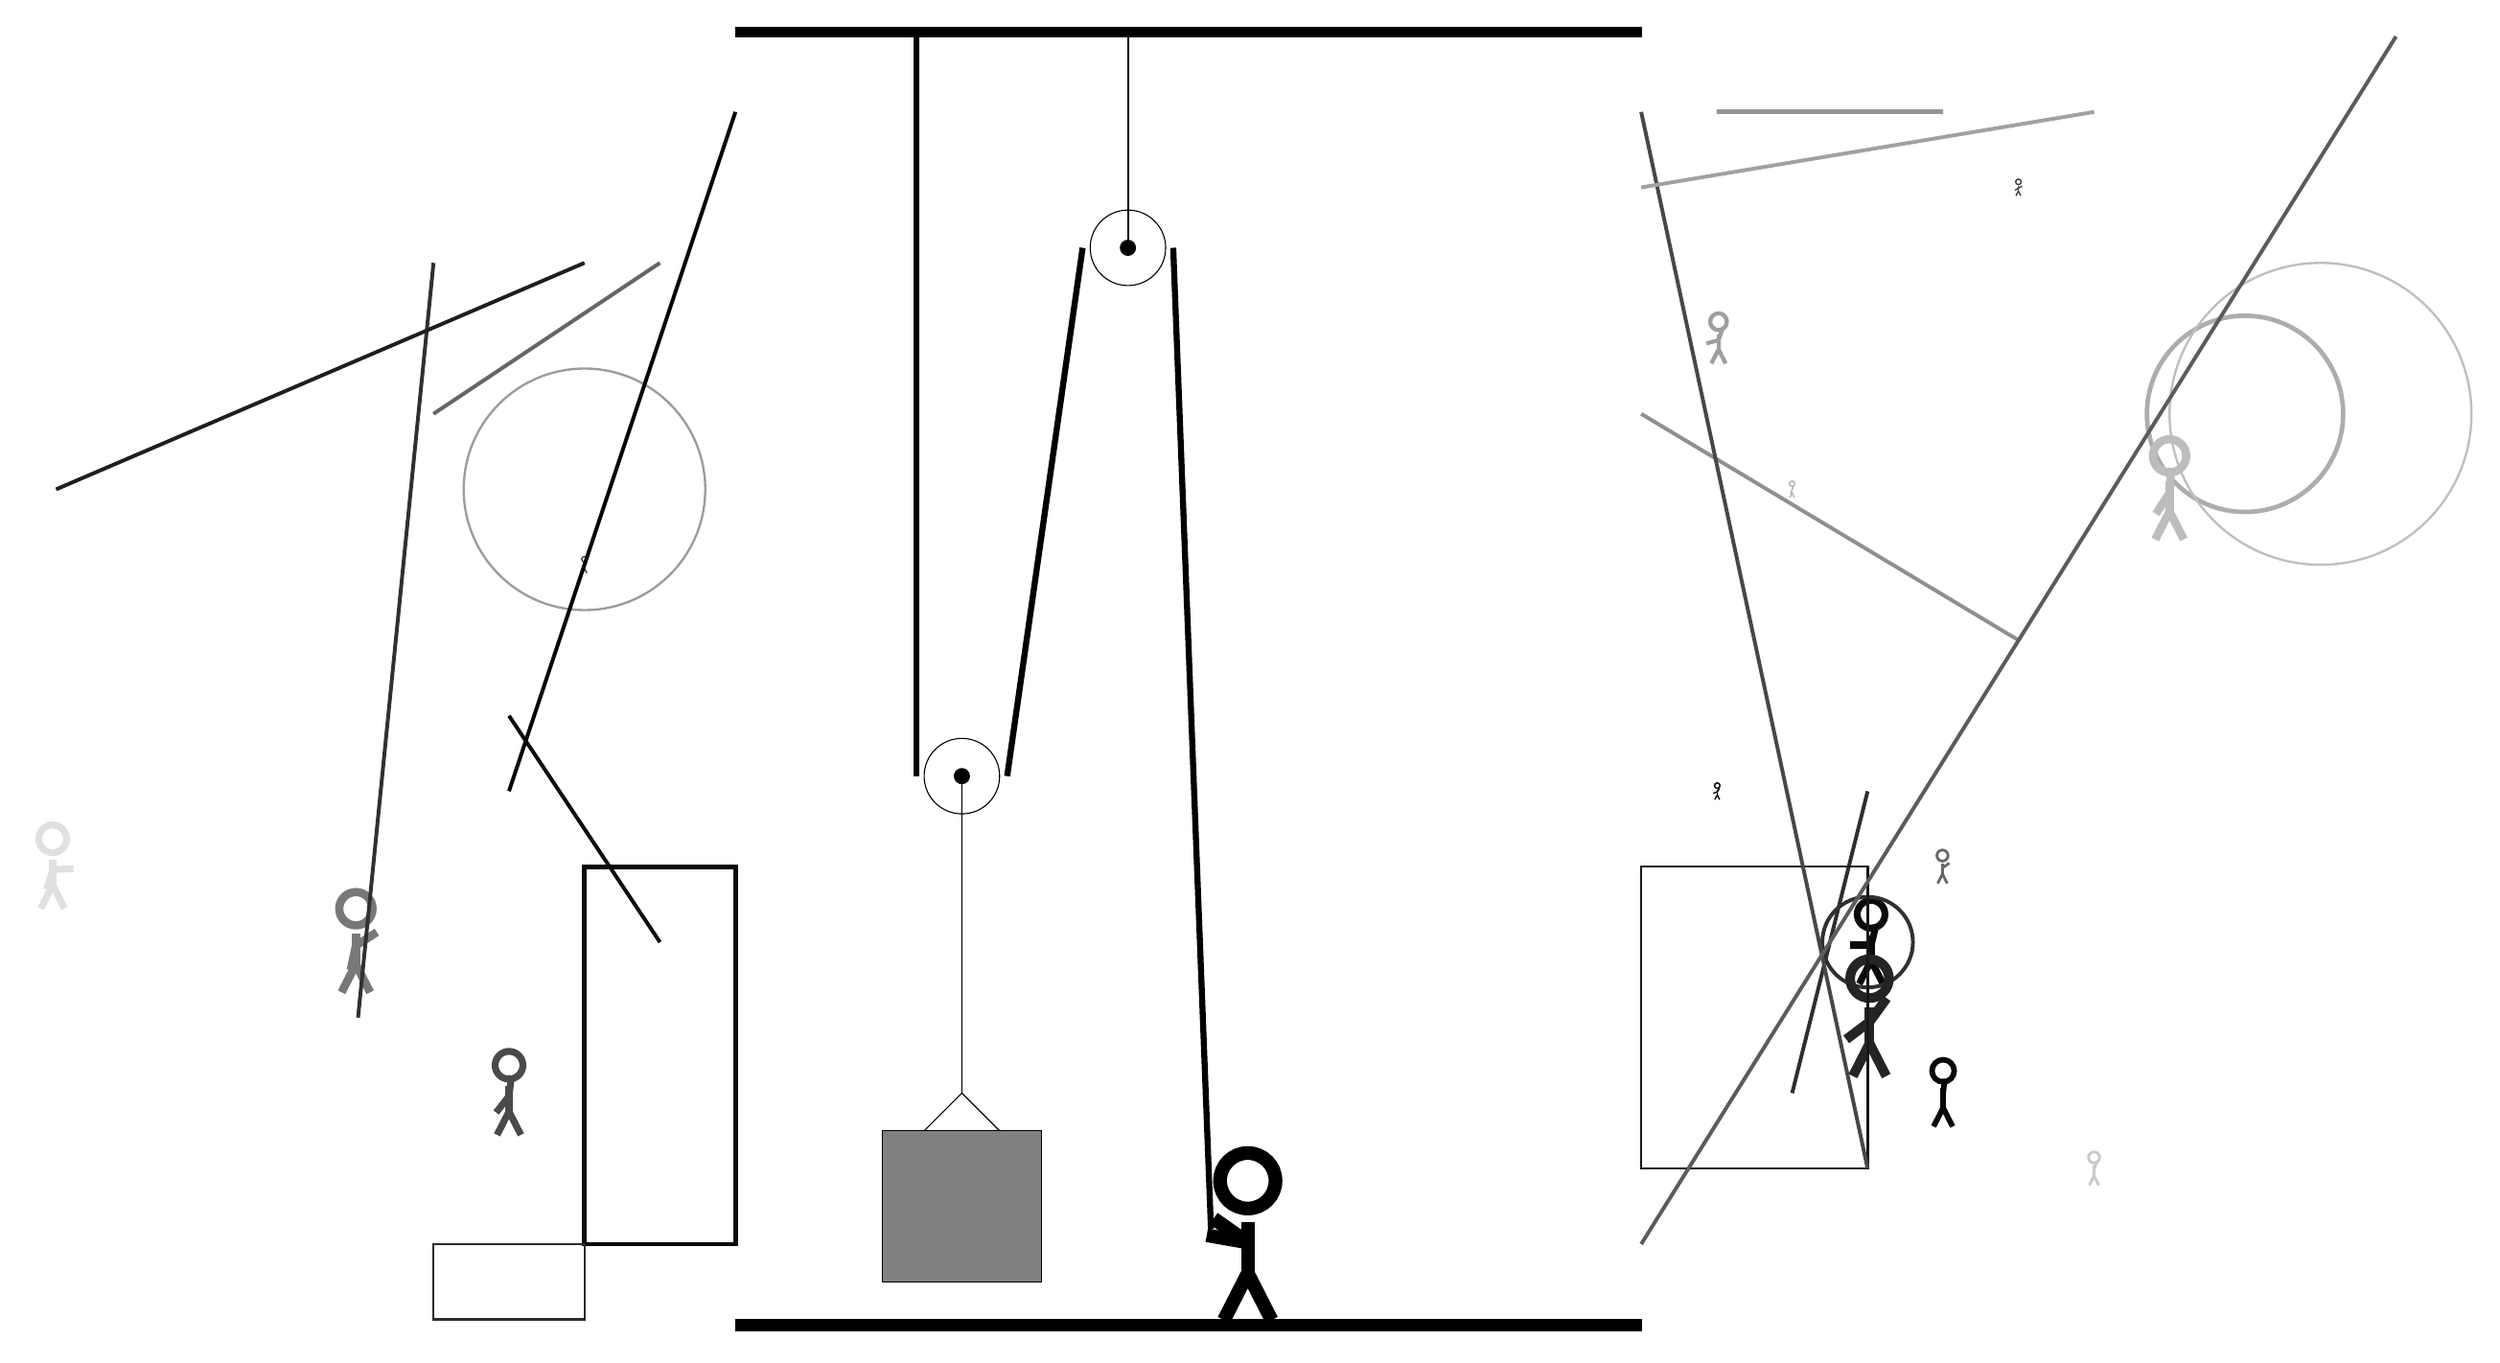
\begin{tikzpicture}
			%%%%% START %%%%%
			
			\draw[fill=black] (-2, 14) rectangle (10, 14.125);
			
			\draw (3.2, 11.2) circle (0.5);
			\draw[fill=black] (3.2, 11.2) circle (0.1);
			\draw[thick] (3.2, 11.2) -- (3.2, 14);
			
			\draw (1, 4.2) circle (0.5);
			\draw[fill=black] (1, 4.2) circle (0.1);
			
			\draw (1, 4.2) -- (1, 0) -- (0.5, -0.5);
			\draw (1, 0) -- (1.5, -0.5);
			\draw[fill=black!50] (-0.05, -0.5) rectangle (2.05, -2.5);
			
			\draw[line width=0.8mm] (0.4, 14) -- (0.4, 4.2);
			\centerarc[line width=0.8mm](1, 4.2)(180:360:0.6);
			\draw[line width=0.8mm](1.6, 4.2) -- (2.6, 11.2);
			\centerarc[line width=0.8mm](3.2, 11.2)(0:180:0.6);
			\draw[line width=0.8mm](3.8, 11.2) -- (4.3, -1.8);
			
			\node at (4.7, -1.9) {\Strichmaxerl[10][-35][170]};
			
			\node[line width=0.2mm, color=black!96] at (13, 2) {\Strichmaxerl[5][0][76]};
			
			\draw[line width=0.5mm, color=black!82](13, 4) -- (12, 0);
			\draw [line width=0.6mm, color=black!32](18, 9) circle (1.3);
			\node[line width=0.3mm, color=black!38] at (11, 10) {\Strichmaxerl[3][15][71]};
			\node[line width=0.4mm, color=black!97] at (14, 0) {\Strichmaxerl[4][90][85]};
			
			\draw [line width=0.5mm, color=black!81](13, 2) circle (0.6);
			\node[line width=0.3mm, color=black!86] at (13, 1) {\Strichmaxerl[7][37][54]};
			
			\draw[line width=0.5mm, color=black!96](-3, 2) -- (-5, 5);
			\draw[line width=0.5mm, color=black!44](10, 9) -- (15, 6);
			\draw[line width=0.3mm, color=black!91] (10, -1) rectangle (13, 3);
			\node[line width=0.7mm, color=black!72] at (-4, 7) {\Strichmaxerl[1][90][63]};
			\node[line width=0.7mm, color=black!59] at (14, 3) {\Strichmaxerl[2][89][35]};
			\node[line width=0.2mm, color=black!21] at (16, -1) {\Strichmaxerl[2][87][71]};
			\node[line width=0.2mm, color=black!71] at (-5, 0) {\Strichmaxerl[5][52][83]};
			\draw [line width=0.3mm, color=black!39](-4, 8) circle (1.6);
			\draw[line width=0.5mm, color=black!98](-5, 4) -- (-2, 13);
			
			\draw[line width=0.5mm, color=black!60](-3, 11) -- (-6, 9);
			
			\node[line width=0.4mm, color=black!98] at (11, 4) {\Strichmaxerl[1][21][56]};
			\draw[line width=0.5mm, color=black!72](13, -1) -- (10, 13);
			\node[line width=0.5mm, color=black!53] at (-7, 2) {\Strichmaxerl[6][78][33]};
			\draw[line width=0.5mm, color=black!81](-6, 11) -- (-7, 1);
			
			\draw[line width=0.6mm, color=black!41] (11, 13) rectangle (14, 13);
			\node[line width=0.6mm, color=black!75] at (15, 12) {\Strichmaxerl[1][35][25]};
			\draw[line width=0.6mm, color=black!97] (-4, -2) rectangle (-2, 3);
			\node[line width=0.6mm, color=black!29] at (12, 8) {\Strichmaxerl[1][70][76]};
			
			\draw [line width=0.3mm, color=black!25](19, 9) circle (2.0);
			
			\draw[line width=0.5mm, color=black!37](10, 12) -- (16, 13);
			\draw[line width=0.5mm, color=black!88](-4, 11) -- (-11, 8);
			\draw[line width=0.3mm, color=black!83] (-4, -2) rectangle (-6, -3);
			\node[line width=0.4mm, color=black!12] at (-11, 3) {\Strichmaxerl[5][73][3]};
			\draw[line width=0.5mm, color=black!64](10, -2) -- (20, 14);
			
			\node[line width=0.6mm, color=black!26] at (17, 8) {\Strichmaxerl[6][57][86]};
			
			\draw[fill=black] (-2, -3) rectangle (10, -3.15);
			
			%%%%% END %%%%%
		\end{tikzpicture}
	\end{figure}	
\end{document}